\documentclass[11pt,a4paper,titlepage]{article}

%%%%%%%%%
%%usees%%
%%%%%%%%%
\usepackage[utf8]{inputenc}
%\usepackage[ngerman]{babel}
\usepackage{setspace}
\usepackage{graphicx}
\usepackage{amssymb} 
\usepackage{amsmath}
\usepackage{mathtools}
\usepackage{footnote}
\usepackage{caption}
\usepackage{color}
\usepackage{hyperref}
\usepackage{cite}




%%%%%%%%%
%%Title%%
%%%%%%%%%
\author{Frederik Zwilling 304314}
\title{Proposal:\\ Bachelorthesis Simulation LLSF with Gazebo}
\begin{document}
\maketitle
\thispagestyle{empty}
\tableofcontents
\newpage
\onehalfspace

%%%%%%%%%
%%Text%%
%%%%%%%%
\abstract{Short description}
\section{Introduction}
Autonomous robots are about to play an important role in the future of logistics. They will be able to save time and cost in the industrial production process and boost the economy. Especially multi-robot-systems play an important role in this context. Though, the development of these logistic robots can be difficult because the robots have to handle many complex tasks. They have to detect objects, localize themselves, make a plan of what to do in which order, coordinate with other robots, optimize the work flow, be save for humans and hardware at every time and much more.\\
The key to effective and time saving development of reliable software for robots is simulation. Simulation makes it possible to virtually test written code fast in different scenarios.This leads to better quality of the software and better performance of the robot. By simulating the behavior of a robot much time can be saved because there is no real robot which has to be set up and the simulation can quickly change between different scenarios. Furthermore it is possible to speed the simulation up or run multiple simulations at once. Simulation also makes testing possible if no real robot is available and can be easily used to compare different versions of the software. For example this can be useful to find unknown parameters like thresholds.\\
The proposed bachelor-thesis will work on this area and will develop a simulation environment for the \textit{Logistic League Sponsored by Festo} (LLSF) with the open source simulator \textit{Gazebo} \textcolor{red}{(mulit robot?)}.\\
The Logistic League Sponsored by Festo is part of the \textit{RoboCup
}, an international robotics competition~\footnote{More information can be found at \url{http://www.robocup.org/}}. LLSF aims to catalyze scientific work on autonomous solutions for logistics. The participants should find new approaches and improve already existing ones to optimize material and information flow in the industrial production. LLFS is realized in a fictional production hall. Figure 1 shows this hall and the basic elements.
\begin{figure}
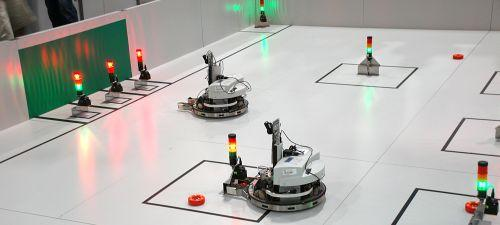
\includegraphics[scale=0.7]{pics/llsf1}
\label{Figure 1}
\caption{A half of the LLSF field. The lights, which look like traffic lights, \textcolor{red}{refferenz schrecklich~\cite{LLSFGermanOpen}}}
\end{figure}


\section{Gazebo}
\section{Related Work}
\section{Detail}
\section{Timetable}
\section{Evaluation}
\section{Conclusion}

\bibliographystyle{plain}
\bibliography{references}

\end{document}
